\documentclass[11pt,a4paper]{article}
\usepackage[a4paper,hmargin=1in,vmargin=1in]{geometry}
\usepackage{pgfplots}
\pgfplotsset{compat=1.17}

\usepackage[czech]{babel}
\usepackage[utf8]{inputenc}
\usepackage[T1]{fontenc}

\usepackage{stddoc}
\usepackage{lipsum}
\usepackage{subcaption}

\newcommand{\plus}{{\texttt{+}}}
\renewcommand{\Re}{\operatorname{Re}}
\renewcommand{\Im}{\operatorname{Im}}
\newcommand{\fourier}[3]{\mathcal{F}_{#1}\!\left[#2\right]\!\left(#3\right)}
\newcommand{\ifourier}[3]{\mathcal{F}^{-1}_{#1}\!\left[#2\right]\!\left(#3\right)}


\begin{document}

\pagenumbering{arabic}

% Header
\noindent\LARGE\textbf{Antennas - theoretical questions}\normalsize\\
\noindent\rule{14.5cm}{0.4pt}

\section{Wire antennas}
\begin{enumerate}
    \item \emph{Units of all quantities}\\
    $[E] = \mathrm V/\mathrm m$, $[H] = \mathrm A/\mathrm m$, $[Z] = \mathrm{\Omega}$, directivity and gain $[D] = [G] = \mathrm{dB}$, $[S] = \mathrm W/\mathrm m^2$

    \item \emph{What is the directivity of isotropic antenna (in linear scale and \emph{dBi})?}\\
    $D = 0 \;\mathrm{dBi} = 1$

    \item \emph{Describe antenna as a filter (in which domains does it filter) and a transformer of waves from guided to waves in free space.}\\
    Antenna behaves like a passive filter in both frequency and spatial domain. It transforms guided waves from a waveguide into radiates waves propagating in free space.

    \item \emph{When an antenna is electrically small and large (in terms in $ka$)? Give examples of such antennas.}\\
    An electrically small antenna is an antenna with $ka \in (0.5, 1)$, where $k = 2\pi/\lambda$ is the wave number. En example of an electrically small antenna is the antenna of Titanic: physical length of $50 \; \mathrm m$ with $f = 500 \; \mathrm{kHz}$.

    \item \emph{What characterizes a TEM transmission line (impedance and operation with frequency)? Sketch distribution of E and H in (a) coaxial line, (b) rectangular waveguide with TE10 mode, (c) microstrip line.}\\
    A truly TEM transmission line in non-disperive meaning that its parameters such as characteristic impedance and phase velocity don't change with frequency. Such TEM mode exists in a coaxial line on all frequencies or in a microstrip line (quasi-TEM) under a specified \emph{cut-off frequency}. In metallic waveguides such as a rectangular waveguide, TE/TM modes propagate above respective cut-off frequencies.
    \begin{figure}[!ht]
        \centering
    \begin{subfigure}{0.45\textwidth}
        \centering
        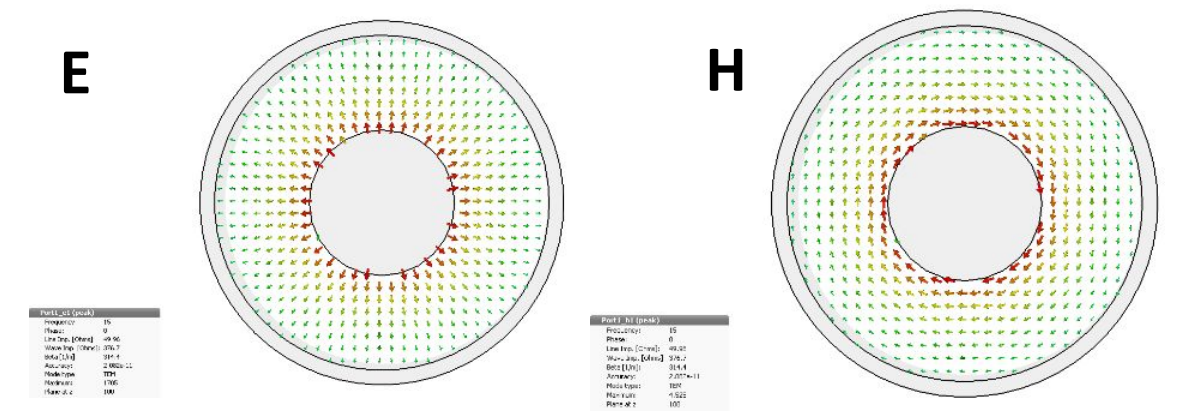
\includegraphics[width=\textwidth]{src/tem-coax.png}
        \caption{Coaxial TEM}
    \end{subfigure}
    \begin{subfigure}{0.45\textwidth}
        \centering
        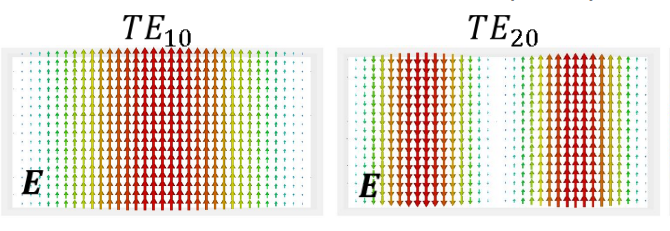
\includegraphics[width=\textwidth]{src/te-rectangular.png}
        \caption{Rectangular TE}
    \end{subfigure}\\
    \begin{subfigure}{0.9\textwidth}
        \centering
        
\includegraphics[width=\textwidth]{src/tem-microstrip.png}
        \caption{Microstrip TEM}
    \end{subfigure}
    \caption{Propagation modes in different transmission lines}
    \end{figure}

    \item \emph{Sketch circuit model of a transmitting and receiving antenna.}\\
    \begin{figure}[!ht]
        \centering
        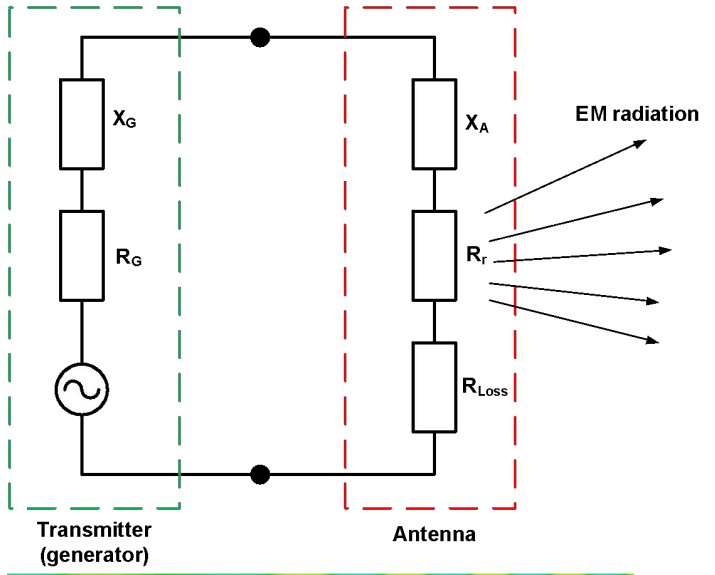
\includegraphics[width=0.6\textwidth]{src/circuit-model.png}
        \caption{Question 6}
    \end{figure}

    \item \emph{What is radiation resistance and radiation efficiency? Radiation efficiency of electrically small antennas.}\\
    Radiation resistance is the equivalent resistance accounting for the signal loss due to radiation.\\
    Radiation efficiency ($\eta = R_r/(R_r+R_{\mathrm{Loss}})$) is the ratio of the radiated power to the total power supplied to the antenna. Electrically small antennas tend to have small radiation efficiency.

    \item \emph{Define VSWR, Return Loss and relative bandwidth.}\\
    Voltage Standing Wave Ratio: $\mathrm{VSWR} = (1+|\Gamma|)/(1-|\Gamma|)$, where $\Gamma = (Z_L - Z_0)/(Z_L + Z_0)$ is the reflection coefficient.\\
    Return Loss: $\mathrm{RL} = -20\log_{10}|\Gamma|$ in dB.\\
    Relative bandwidth: $\mathrm{BW} = (f_2 - f_1)/f_0 = (f_2 - f_1)/\sqrt{f_1f_2}$.

    \item \emph{What is the physical meaning of the free space Green's function?}\\
    The free space Green's function corresponds to the one of a spherical wave.

    \item \emph{Elementary electric dipole - what field components it does have (if z-oriented) in near and far field? What is its farfield pattern and why it is not isotropic even for dipole length approaching 0.}
    \begin{itemize}
        \item Near (reactive) field region $kr \ll 1$: Fields are similar to those of a static electric dipole and to the of a static current element. $E_r$ and $E_\theta$ are out-of-phase with $H_\varphi$. There is no time-average power flow nor radiated power; energy is stored in the near-zone.
        
        \item Intermediate field region $kr > 1$: Field are similar to those of a static electric dipole and to the of a static current element (quasistationary fields). $E_\theta$ and $H_\varphi$ approach time-phase which means the beginning of time-average power flow in the outward (radial) direciton.
        
        \item Farfield region $kr \gg 1$: Most important region of an antenna. $E_r$ vanishes and only transversal (to $r$) field components ($E_\theta$ and $H_\varphi$) remain.
    \end{itemize}
    It can't be isotropic even for dipole length approaching 0 due to the projection $\sin(\theta)$. Magnetic dipole has farfield components $E_\varphi$ and $H_\theta$.

    \item \emph{Define radiation intensity and antenna directivity. Directivity vs electrical size of antenna. Radiation pattern properties (sidelobe level, front-to-back ratio, half power beamwidth, polarization).}\\
    Radiation intensity $U$ is defined as the power radiated from an antenna per unit space angle (in steradians) and is related to the farfield $E$ of the antenna:
    \begin{align*}
        U(\theta,\varphi) = r^2S(\theta,\varphi) = \frac{r^2}{2Z_0} \norm{E(\theta,\varphi)}^2.
    \end{align*}
    Directivity is the ratio of the radiation intensity in a given direction from the antenna to the radiation intensity averaged over all directions, i.e., isotropic source:
    \begin{align*}
        D(\theta,\varphi) = \frac{U(\theta,\varphi)}{U_0} = \frac{4\pi U(\theta,\varphi)}{P_r}.
    \end{align*}
    Maximum directivity is then given by
    \begin{align*}
        D_{\mathrm{max}} = \frac{U_{\mathrm{max}}}{U_0} = \frac{4\pi}{\oint_S f_n^2(\theta,\varphi) \; \d S}.
    \end{align*}
    For example for the elementary electric dipole, $f_n(\theta,\varphi) = \sin(\theta)$ and $D_{\mathrm{max}} = 3/2$ in linear scale which corresponds to $10\log(3/2) \; \mathrm{dBi} \approx 1.76 \; \mathrm{dBi}$.\\
    Sidelobe level: radiation intensity level of the most significant sidelobes.\\
    Front-to-back ratio: power ratio of the main lobe to the back lobe.\\
    HPBW: bandwidth across which half of the power is radiated.\\
    Polarization is defined as the property of an EM wave describing the time-varying direction and relative magnitude of $\vec E$. Most common types are linear and circular (LHC/RHC).

    \item \emph{Can we speak about farfield if an antenna is embedded in an lossy space of infinite background?}\\
    We cannot since the radiation pattern is defined on a sphere with the radius approaching infinity. Thus it does not make sense to speak about it in a lossy environment.

    \item \emph{How to evaluate radiation resistance from radiation pattern and are there other possibilities?}\\
    One possibility is to integrate the Poynting vector $\vec S$ over a closed surface around the antenna to obtain the radiated power $P_r = I^2 R/2$ from which we can obtain the radiation resistance $R$.\\
    An alternate way is to calculate the radiated power $P_r$ using source currents instead of fields.

    \item \emph{What is EIRP?}\\
    EIRP stands for effective isotropic radiated power and it is the total power which must be radiated by an isotropic antenna in order for it to yield the same radiation intensity in a given direction. The units of EIRP are watts (W).

    \item \emph{Explain the physical meaning of the following integral:}
    \begin{align*}
        \vec A(\vec r) = \frac{\mu}{4\pi} \int_{V'} \vec J(\vec r') \frac{e^{-ikR}}{R} \; \d V'
    \end{align*}
    The integral states that the field vector potential is a sum of contributions in the form of source currents $\vec J$ multiplied by the Green's function of a spherical wave.

    \item \emph{Mark $r$ terms which contribute to near and far field. Which antenna does produce these fields? What is its orientation in cartesian cordinates?}
    \begin{align*}
        H_{\varphi}(r,\theta) &= \frac{ikIL}{4\pi} \sin(\theta) \bigg[ \underbrace{\frac 1r}_{\mathrm{farfield}} + \underbrace{\frac{1}{ikr^2}}_{\mathrm{nearfield}} \bigg] e^{-ikr},
    \\
        E_r(r,\theta) &= \frac{Z_0IL}{2\pi} \cos(\theta) \bigg[ \underbrace{\frac{1}{r^2}}_{\mathrm{nearfield}} + \underbrace{\frac{1}{ikr^3}}_{\mathrm{nearfield}} \bigg] e^{-ikr},
    \\
        E_\theta(r,\theta) &= \frac{ikZ_0IL}{4\pi} \sin(\theta) \bigg[ \underbrace{\frac 1r}_{\mathrm{farfield}} + \underbrace{\frac{1}{ikr^2}}_{\mathrm{nearfield}} - \underbrace{\frac{1}{k^2r^3}}_{\mathrm{nearfield}} \bigg] e^{-ikr},
    \\
        H_r &= H_\theta = 0,
    \\
        E_\varphi &= 0.
    \end{align*}
    From simple vanishing properties of polynomials: only the terms of order $-1$ don't vanish in farfield. The above is the solution for the elementary electric dipole oriented in the $z$-axis and its length approaches 0.

    \item \emph{Current distribution on linear (wire) antenna, what approximations are used (constant, triangular and sinusoidal current)?}\\
    Assuming $z$-axis orientation (thin antenna), the distributions take form of
    \begin{align}
        \tag{Triangular}
        I(z) &= I_0\(1 - \frac{2|z|}{L}\),
    \\
        \tag{Sinusoidal}
        I(z) &= I_0 \sin\(k\(\frac L2 - |z|\)\).
    \end{align}
    For the length $L = 0.5\lambda$, we obtain the sinusoidal distribution. The triangular distribution arises for smaller dipoles, whereas the constant distribution concerns the elemental dipole.

    \item \emph{Sketch current distribution at dipoles of lengths $0.1\lambda$, $0.5\lambda$, $1\lambda$, $1.25\lambda$, $2\lambda$, \dots What effect do out-of-phase currents have on farfield?}\\
    \begin{figure}[!ht]
        \centering
        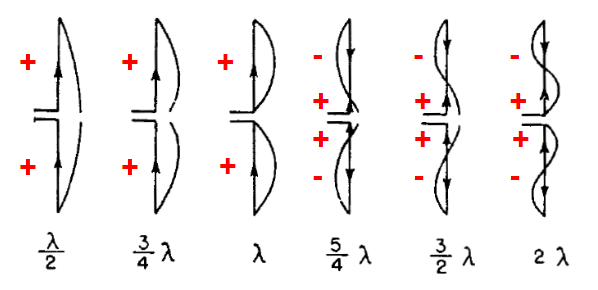
\includegraphics[width=0.8\textwidth]{src/dipole-lengths.png}
        \caption{Current distributions for different dipole lengths}
    \end{figure}
    Out-of-phase currents (caused by $L > \lambda$) produce sidelobes in the farfield.\\
    Missing distribution of $L = 0.1\lambda$: triangular distribution.

    \item \emph{Evaluation of near and far field of linear antennas - far field approximation, Fourier transform between current and far field, polarization projections, \dots}\\
    The farfield approximation revolves around the expression
    \begin{align*}
        R \approx r - \Delta = r - z' \cos(\theta) = r - \vec r' \cdot \vec e_r.
    \end{align*}
    The $\Delta$ term's contribution can then be neglected in amplitude but not in phase. This approximation leads to the useful conclusion that the radiated field is directly proportional to the Fourier transform of the source currents.

    \item \emph{Directivity of linear antennas ($1.25\lambda$ dipole)}
    \begin{figure}[!ht]
        \centering
        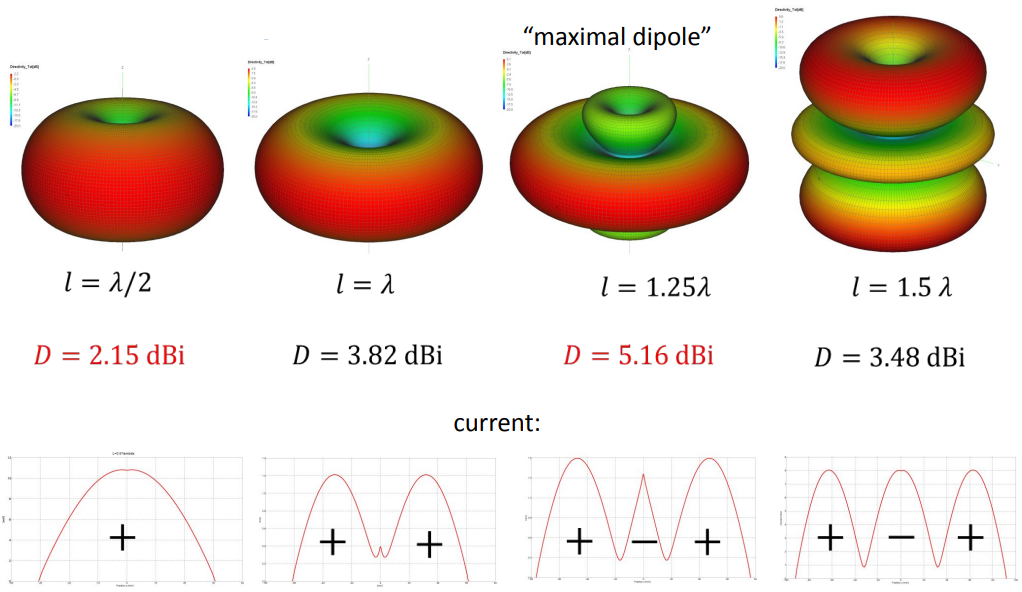
\includegraphics[width=0.8\textwidth]{src/dipole-radiation-patterns.png}
        \caption{Radiation patterns}
    \end{figure}

    \item \emph{$\lambda/2$ dipole properties (input impedance, pattern), shortening to resonance, bandwidth}\\
    Radiation pattern: omnidirectional in the $H$-plane which is a useful property for many applications including mobile communications.\\
    Directivity: reasonable value (2.15 dBi), larger than of short dipoles.\\
    Imput impedance: $~73 \; \Omega$ which is pretty much well matched with a standard transmission line of characteristic impedance of $75 \; \Omega$; not sensitive to changes in the radius of the dipole.\\
    Shortening: the dipole itself is not exactly resonant and hence should be shortened by a little amount, depending on the radius.\\
    Bandwidth: connected to its input impedance; 5 to 15 \% from the central frequency.

    \item \emph{Folded $\lambda/2$ dipole - impedance, pattern}\\
    Its impedance is about 4 times of the normal dipole which significantly increases its bandwidth. The pattern is similar to the normal dipole I think?

    \item \emph{Symmetrization, baluns}\\
    Symmetrization problem arises when connecting an unbalanced transmission line to the antenna. The balanced mode is when there are equal and opposite currents.\\
    Balun transforms the balanced input impedance of the dipole to the unbalanced impedance of the coaxial line such that there is no net curernt on the outer conductor of the coax.\\
    Further comments: non-symmetrical feeders are cheaper and simpler but require a symmetrization unit (balun) for connection to the symmetrical antenna.

    \item \emph{Monopole antennas (impedance, pattern compared to dipoles), method of images}\\
    Impedance: roughly half the dipole version\\
    Gain: roughly double (+3 dBi)\\
    Pattern: radiates only above ground\\
    Method of images: replacement of the ideally infinite ground plane by an opposite electrode creating dipole structure for radiation. Realistically, we use radial lines (pieces of wires) instead of the ideal infinite ground plane.

    \item \emph{Horizontal dipole above ground - method of images}\\
    By superposition, the ground plane above which the horizontal dipole sits can be modelled by a virtual image dipole with opposite current feed in the halfspace below ground plane.

    \item \emph{Explain what the terms in braces physically represent:}
    \begin{align*}
        E_\theta(r,\theta,\varphi) &= \underbrace{\frac{ikZ_0}{4\pi} \frac{e^{-ikr}}{r} \sin(\theta)}_A \underbrace{\int_{-l/2}^{l/2} I_z(z') e^{ikz' \cos(\theta)} \; \d z'}_B
    \end{align*}
    A: element factor (elementary dipole contribution)\\
    B: space factor (Fourier transform of the source)

    \item \emph{Aperture antennas - equivalent source approach}\\
    First, we envelop the antenna with a closed surface because we are interested in the field far beyond the antenna, not the field nearby. Then we substitute the sources distributed inside the closed surface ("volume of the antenna") by sources only on the surface. These currents must be so that they produce the same field around the antenna. Lastly we set the fields inside equal to zero which alters the field inside where we don't care. 
    
    \item \emph{Aperture in infinite ground plane and in free space - what equivalent sources to use?}\\
    Infinite ground plane: $\vec M = -2\vec n \times \vec E$.\\
    Free space: $M = -\vec n \times \vec E$ and $\vec J = \vec n \times \vec H$. Additionally we demand that the feeding waveguide contains a TEM wave.
    
    \item \emph{Physical meaning of radiation integrals in near and far field. Far field distance, conditions for far field ($1/r$ dependence, $E/H$ ratio, transversal fields)}\\
    Aperture radiation can be imagined as the radiation of an infinite number of point sources placed in the aperture. The radiation integrals are a superposition of these sources' contributions.\\
    For nearfield, we need a numerical solution using original sources. Farfield described as distance greater than $2D^2/\lambda$, where $D$ is the maximal dimension of the antenna, allows for approximation which yields analytical solution. In farfield, impedance is equal to the impedance of the free space $Z = E/H = 120\pi \approx 377 \; \Omega$.
    
    \item \emph{Structure of the far field (Fourier transform $\times$ obliquity factors). Relation to array.}\\
    In farfield, the field can be expressed as the Fourier transform of the sources multiplied by obliquity factors, which include projection from Cartesian to spherical coordinates and a relation between $E$ and $H$.

    \item \emph{Huygens source properties, element factor.}\\
    Aperture antennas which can be considered Huygens sources have the virtue of perpendicular electric and magnetic fields. Furthermore:
    \begin{itemize}
        \item $E/H = Z_0 = 120\pi$,
        \item locally a plane wave,
        \item radiation pattern is a cardioid,
        \item element factor $(1+\cos(\theta))/2$.
    \end{itemize}

    \item \emph{Far field of aperture with constant (amplitude, phase) source field}\\
    Can be expressed as the product of Fourier transforms of the repsective distributions along $x$ and $y$? I don't have a decent answer\dots

    \item \emph{Directivity of aperture antennas (effective area)}\\
    Directivity of aperture antennas can be easily computed using the effective area:
    \begin{align*}
        D_{\mathrm{max}} = \frac{4\pi U_{\mathrm{max}}}{\lambda^2} \frac{\left| \int_{S_A} \vec E_a(x',y') \; \d x' \d y' \right|^2}{\int_{S_A} \norm{\vec E_a(x',y')}^2 \; \d x' \d y'} = \frac{4\pi U_{\mathrm{max}}}{\lambda^2} A_{\mathrm{eff}}.
    \end{align*}
\end{enumerate}

\section{Horn antennas}
\begin{enumerate}
    \item \emph{Field distribution in rectangular waveguide with the TE10 mode, amplitude and phase at its aperture}
    \item \emph{Why its radiation pattern differs in its E and H plane?}
    \item \emph{1D aperture with linear and quadratic phase - effects on pattern. Quadratic phase error - where it appears}
    \item \emph{Horn antennas - basic properties, why we use them and for what}
    \item \emph{Phase effects in the aperture of a horn}
    \item \emph{Directivity vs aperture size (phase distortion), optimal horn, aperture efficiency}
    \item \emph{What is phase center of a horn antenna}
    \item \emph{Horns with mixed modes in aperture, why we do that. Polarization of horn antennas}
    \item \emph{Explain far field approximation of the Green's function $\operatorname{exp}(-ikR)/R$ using picture below:}
    \begin{figure}[!ht]
        \centering
        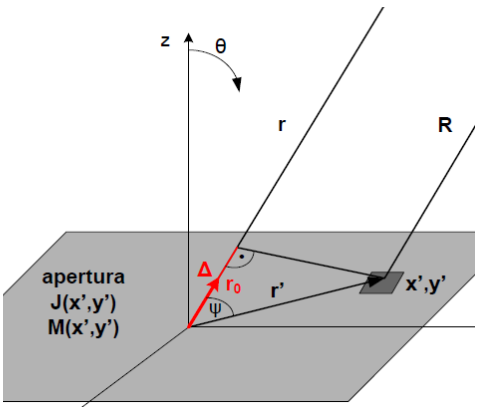
\includegraphics[width=0.7\textwidth]{src/farfield-approximation.png}
        \caption{Question 11}
    \end{figure}
    \item \emph{What does this integral physically mean and where is it used?}
    \begin{align*}
        \vec P(\theta,\varphi) &= \int_S \vec E_a(x',y') e^{ik(x'\sin(\theta)\cos(\varphi) + y'\sin(\theta)\sin(\varphi))} \; \d x' \d y'
    \end{align*}
    \item \emph{Explain all the terms in the following equation. What does this equation represent?}
    \begin{align*}
        E_\theta(\theta,\varphi,r) &= \frac{iE_0ab}{\lambda} \frac{e^{-ikr}}{r} \frac{1+\cos(\theta)}{2} \sin(\varphi) \frac{\sin\(k_x \frac a2 \)}{k_x \frac a2} \frac{\sin\(k_y \frac b2 \)}{k_y \frac b2}
    \end{align*}
    \item \emph{What is this graph about?}
    \begin{figure}[!ht]
        \centering
        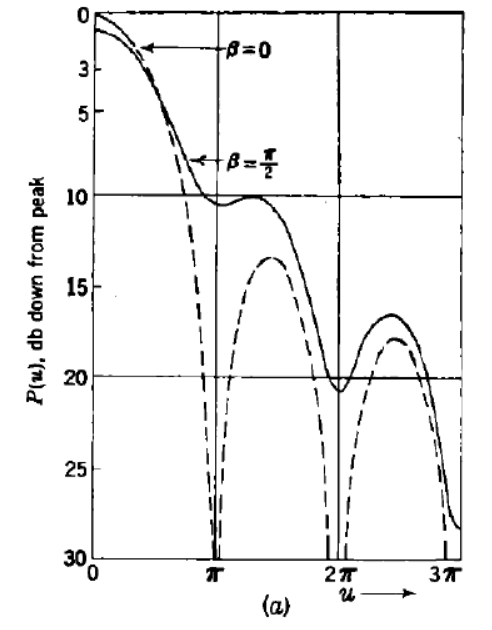
\includegraphics[width=0.7\textwidth]{src/what-is-this-graph.png}
        \caption{Question 14}
    \end{figure}
    \item \emph{Why we use parabolic reflector antenna, what is its physical principle?}
    \item \emph{What happens if the feed is off the focus of the parabolic reflector antenna?}
    \item \emph{Explain (sketch) illumination and spillover loss in the parabolic reflector antenna.}
    \item \emph{What is typical aperture efficiency of the parabolic reflector antenna? What edge taper corresponds to the maximum efficiency?}
    \item \emph{What are the properties of an "ideal" feed for parabolic reflector antenna?}
    \item \emph{What effects mostly contribute to the antenna noise antenna temperature?}
\end{enumerate}

\end{document}